\documentclass[a4paper,12pt]{report}
\usepackage{xcolor}
% Lingua e codifica
\usepackage[utf8]{inputenc}
\usepackage[T1]{fontenc}
\usepackage[english]{babel}
\usepackage{graphicx}
\usepackage{multirow}


% Impostazioni della pagina
\usepackage[margin=2.5cm]{geometry}
\usepackage{setspace}
\onehalfspacing

% Immagini, formule e tabelle
\usepackage{graphicx}
\usepackage{amsmath}
\usepackage{booktabs}

% Collegamenti e indice cliccabile
\usepackage[
    colorlinks=true,
    linkcolor=blue,
    urlcolor=blue,
    filecolor=blue
]{hyperref}

% Dati del report: modifica qui
\title{RAG System \\[0.5cm]
       \large Architectural Design and Implementation}
\author{Giovanni De Francesco \\ \
        \small Università degli Studi di Napoli Federico II \\[0.5cm]
        \small Text Mining Exam}
\date{\today}

\begin{document}

% Copertina
\maketitle

% Indice automatico
\tableofcontents
\clearpage













\chapter{Introduction}
This report presents the design and implementation of a
Retrieval-Augmented Generation (RAG) system, outlining the project
objectives, methodology, experimental results, and main conclusions.

The study investigates two RAG architectures:
\begin{itemize}
    \item a single-agent architecture;
    \item a multi-agent architecture.
\end{itemize}

Each architecture is evaluated in two configurations:
\begin{enumerate}
    \item \textbf{Without LangChain:} the system is implemented
    without the LangChain framework and uses a specific embedding
    model.
    \item \textbf{With LangChain:} the system is implemented using
    the LangChain framework and a different embedding model.
\end{enumerate}

\section{Context}

Both architectures use a reference dataset called
\textit{Context Data}, which consists of three country-specific
subsets: Italy, Estonia, and Slovenia.

\subsection{Dataset Structure}

For each country, the corpus is organized into three main
content categories:
\begin{itemize}
    \item \textbf{Inheritance law:} civil code provisions governing
    inheritance and succession.
    \item \textbf{Divorce and family law:} civil code provisions
    and related rules governing separation, divorce, and family
    matters.
    \item \textbf{Past legal cases:} case materials concerning
    inheritance and divorce, including court decisions,
    settlements, and mediation outcomes.
\end{itemize}

\subsection{Document Format and Metadata}

All documents are stored in JSON format. Each file contains
a text field holding the content of a legal provision or case,
together with associated metadata.

The metadata typically include the following:
\begin{itemize}
    \item \textbf{Country:} Italy, Estonia, or Slovenia.
    \item \textbf{Legal area:} inheritance or divorce.
    \item \textbf{Referenced provisions:} relevant civil code
    articles, where applicable.
    \item \textbf{Document type:} \texttt{code} for legal provisions
    or \texttt{case} for case materials.
    \item \textbf{Source:} the source from which the document
    was obtained.
\end{itemize}

Additional metadata may describe the duration and cost of
proceedings, the nature of the dispute, and other contextual
information.

















\chapter{RAG Implementations without LangChain}
\label{chap:rag-without-langchain}

This chapter examines single-agent and multi-agent
Retrieval-Augmented Generation (RAG) implementations developed
without LangChain. Both approaches use the same legal document
collection, ingestion pipeline, embedding model, and language model
configuration. This shared foundation supports a comparison of how
architectural differences affect retrieval and answer generation.

Both documents and queries are embedded using
\texttt{BAAI/bge-m3}, which produces 1,024-dimensional vectors.
The following section describes the shared ingestion process.

\section{Shared Document Ingestion Pipeline}
\label{sec:shared-ingestion}

The ingestion pipeline converts legal documents into a searchable
knowledge base used by both implementations. Defined in
\texttt{Ingestion.ipynb}, it consists of five main stages: document
validation, metadata preparation, chunking, embedding generation,
and storage in Pinecone.

\subsection{Document Loading and Metadata Preparation}

The dataset consists of JSON files organized by country and document
category. Each file contains document text and associated metadata.
The pipeline checks the directory structure, parses each file, and
verifies that the document text is non-empty. Loading errors and
missing legal-area values cause processing to stop before uploading
begins.

Each document is assigned metadata identifying its country, legal
area, document type, and source path. Document types are classified
as \texttt{Legal Cases} or \texttt{Civil Codes}. For legislation,
the legal area is derived from the folder name; for judicial
decisions, it is read from the original metadata. Legal-area values
in case metadata must therefore match the vocabulary used by the
retrieval filters.

Citation labels combine the country and legal area with a case
identifier or legislative reference. The filename is used when the
preferred identifier is unavailable. These labels support source
attribution during answer generation and subsequent verification.

\subsection{Chunking and Embedding Generation}

Document text is divided into chunks of up to 1,500 tokens using
the BGE-M3 tokenizer, with an overlap of 150 tokens between adjacent
chunks. Documents shorter than this limit remain intact. The overlap
helps preserve context across adjacent passages, although fixed
token boundaries may split sentences or legal provisions.

BGE-M3 uses a \textbf{subword tokenizer}, which divides rare or
technical terms into smaller recurring units while retaining common
words as single tokens when possible.

Before embedding, each chunk is enriched with a compact header
and its metadata. BGE-M3 then generates a normalized,
1,024-dimensional dense vector for each enriched chunk.

Embedding generation runs on a CUDA-enabled GPU when available
and falls back to the CPU otherwise. During retrieval, the same
model encodes user queries into the same vector space.

\subsection{Vector Storage and Retrieval Integration}

Vectors are uploaded to the shared \texttt{legal-rag} Pinecone
index, which is configured for 1,024-dimensional vectors and
cosine similarity. Each record contains an embedding, source text,
metadata, a citation label, and the chunk's position within the
source document. A deterministic identifier derived from the source
path and chunk position ensures that repeated uploads target the
same record.

Before uploading, the notebook validates the index configuration
and reports document counts. In its current configuration, it clears
the target namespace and rebuilds the collection from the supplied
dataset.

Both the single-agent and multi-agent implementations retrieve
documents from this index using metadata filters. In the
single-agent system, the router determines the search scope.
In the multi-agent system, specialist agents apply filters
corresponding to their respective jurisdictions, legal areas,
and document types.





\section{Single-Agent Workflow}
\label{sec:single-agent-workflow}

Figure~\ref{fig:single-agent-flowchart} illustrates a conversation turn,
from user input to response delivery. Each subsequent message starts
a new turn using the saved conversation context.

The diagram uses blue for memory operations, green for user
interaction, and yellow for internal response preparation.

\begin{figure}[p]
    \centering
    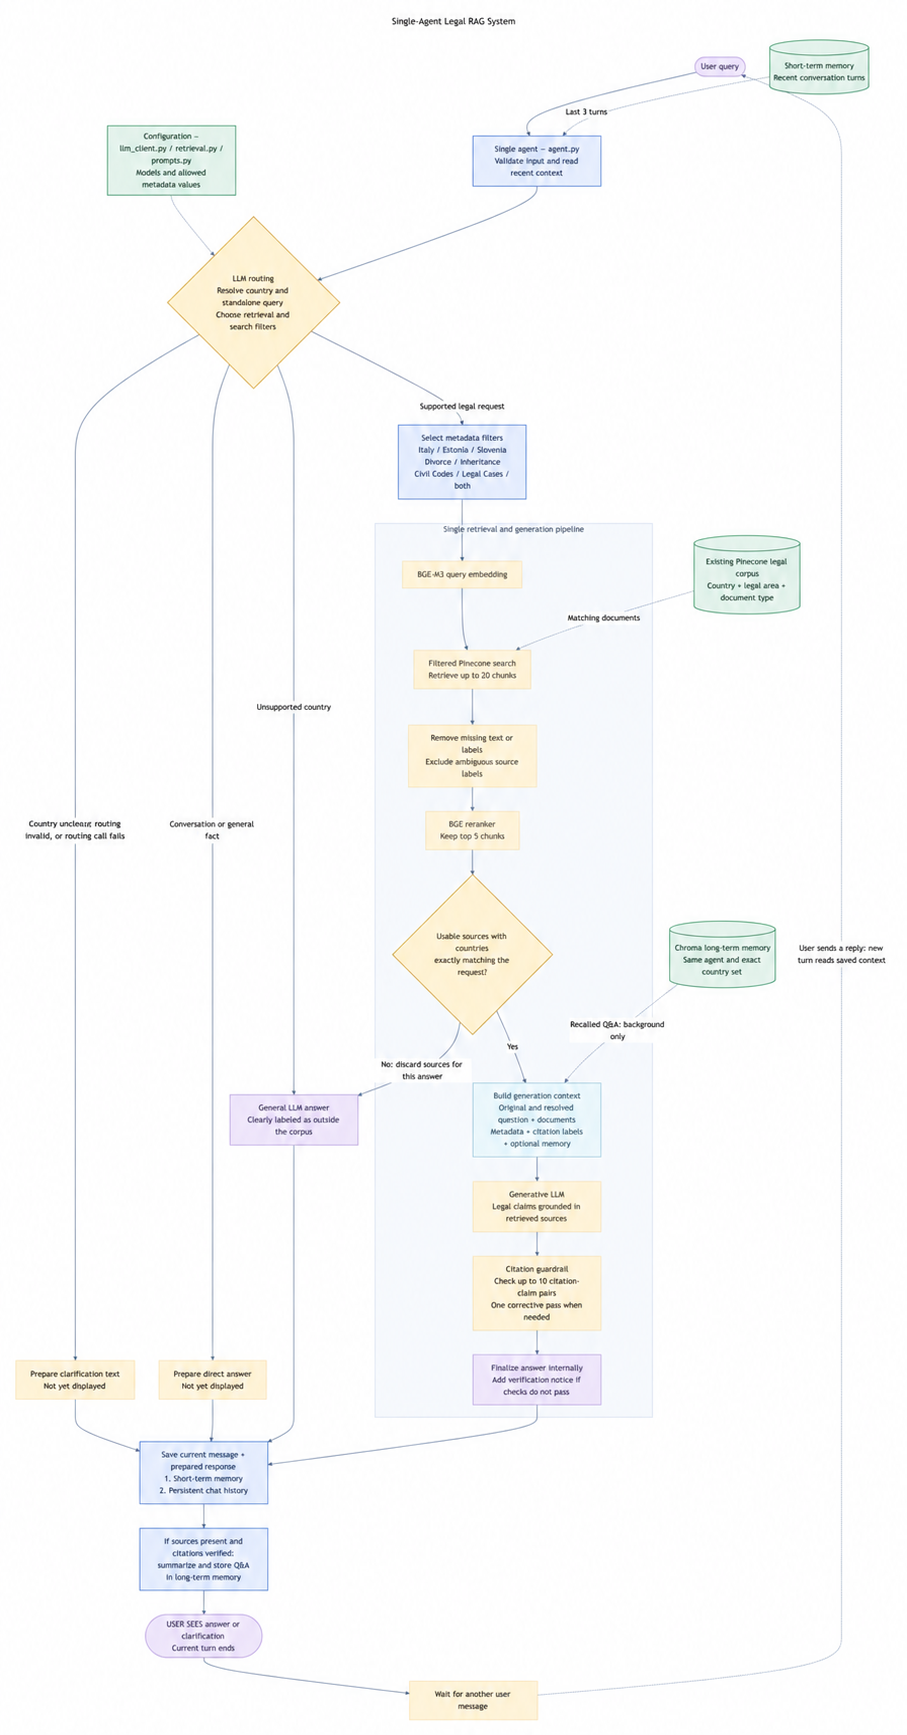
\includegraphics[
        width=\textwidth,
        height=0.85\textheight,
        keepaspectratio
    ]{immagini/single-agent-system.png}
    \caption{Single-agent RAG workflow.}
    \label{fig:single-agent-flowchart}
\end{figure}

\subsection{Input Processing and Routing}

The user submits a question through the Gradio interface. The system
validates the input and reads the last three conversation turns from
short-term memory to interpret follow-up questions.

A single LLM call determines whether retrieval is needed, rewrites
the question as a standalone query, and selects metadata filters.
The diagram separates these operations for clarity. Conversational
requests and general factual questions may receive a direct answer,
while jurisdiction-dependent legal questions favor retrieval.
Unclear jurisdictions, invalid routing responses, or routing-call
failures produce a clarification request.

\subsection{Country Identification and Search Scope}

The router identifies countries from the current question or
unambiguous references in earlier user messages. The corpus covers
Italy, Estonia, and Slovenia. Requests involving unsupported countries
use a general-knowledge LLM fallback, explicitly identified as not
grounded in the retrieved corpus.

For supported requests, the router selects the legal area
(\texttt{Divorce} or \texttt{Inheritance}) and document types.
Explicit case-law requests select \texttt{Legal Cases}; questions
about statutory provisions, rights, obligations, or legal conditions
select \texttt{Civil Codes}. Requests combining rules and judicial
practice, or leaving the source type unspecified, can search both.

\subsection{Retrieval and Reranking}

BGE-M3 encodes the standalone query for a filtered Pinecone search,
which returns up to 20 candidate chunks. Records without usable text
or citation labels are excluded, together with labels shared by
different sources.

The multilingual cross-encoder
\texttt{BAAI/bge-reranker-v2-m3} scores each query--passage pair,
including relevant passage metadata, and retains up to five chunks.

Every retained chunk must contain country metadata, and their combined
country set must exactly match the requested set. Empty results or
incomplete coverage trigger the LLM fallback. This check establishes
jurisdictional coverage, but not coverage of every aspect of the question.

\subsection{Answer Generation and Verification}

When suitable sources are available, the system recalls relevant long-term summaries scoped to the same agent and country set. These summaries provide background context, while retrieved documents serve as the evidence for legal claims.

The answer model receives the original question, its standalone reformulation, recent conversation history, retrieved documents, and recalled summaries. Before the answer is returned to the user, the output guard checks up to ten citation–claim pairs per pass. If it detects citations that are absent from the retrieved sources or claims unsupported by their cited sources, it requests one corrective rewrite and checks the revised answer again. Any remaining issues or incomplete verification are reported in a notice accompanying the answer. Direct answers and fallback answers generated without suitable sources bypass this guard.


\subsection{Storage and Response Delivery}

Each completed turn saves the user message and finalized response
in short-term memory and persistent chat history, including
clarifications, direct answers, and fallbacks. Long-term storage is
attempted only when retrieved documents are present and citation
verification succeeds. The response is then returned to the interface.

For example, \textbf{``How does divorce work?''} may prompt a request
to specify the country. If the user replies \textbf{``Italy''}, the
next turn uses the saved context to reconstruct
\textbf{``How does divorce work in Italy?''} and proceeds through
retrieval and answer generation. The flowchart's return arrow
therefore represents a new user message, rather than an automatic
continuation of the previous turn.




\section{Single-Agent Architecture and Main Modules}
\label{sec:single-agent-architecture}
The single-agent implementation coordinates routing, retrieval,
answer generation, verification, and memory through a single
application controller. Its principal modules are described below.

\subsection{Configuration Management}

The \texttt{llm\_client.py} module centralizes language-model
configuration. It loads environment settings and exposes
\texttt{get\_llm\_client()} and \texttt{model\_names()}, ensuring
consistent configuration across answer generation, citation
verification, and memory summarization.

Retrieval settings specify the Pinecone index and namespace.
Supported countries, legal areas, and document types are defined
in \texttt{retrieval.py}.

\subsection{Document Retrieval and Vector Stores}

The \texttt{PineconeRetriever} class in \texttt{retrieval.py}
provides access to the legal corpus. The
\texttt{build\_metadata\_filter()} function converts the router's
selections into validated metadata filters.

The retriever generates normalized BGE-M3 query embeddings,
searches Pinecone, validates the returned records, and reranks
the candidates using a BGE cross-encoder.

A separate Chroma database, managed by
\texttt{memory/long\_term.py}, stores summaries of previous
question--answer exchanges. It uses \texttt{all-mpnet-base-v2}
embeddings for semantic recall. Pinecone supplies documentary
evidence, while Chroma supplies conversational background.
The application initializes the conversational store without
rebuilding the legal-document index.

\subsection{Answer Coordination}

The \texttt{SingleAgentRAG} class in \texttt{agent.py} coordinates
the workflow through its \texttt{ask()} method.

The \texttt{\_triage\_and\_route()} method determines whether
retrieval is required, resolves contextual references, and selects
metadata filters. Based on this decision, the system responds
directly, requests clarification, or retrieves documents.

When the retrieved sources satisfy the country-coverage check,
\texttt{\_answer\_with\_rag()} generates a response grounded in
those sources. Unsupported jurisdictions, empty retrieval results,
or incomplete country coverage trigger
\texttt{\_answer\_without\_sources()}.

All these paths are managed by a single coordinating agent.
The implementation neither delegates questions to specialist
agents nor aggregates independently generated specialist answers.

\subsection{Memory and Answer Verification}

The \texttt{memory} package manages recent conversation context,
long-term semantic recall, and persistent chat history as separate
components. The router receives the last three turns to interpret
follow-up messages.

The \texttt{guardrails/output\_guard.py} module exposes
\texttt{check\_rag\_answer()}, which checks citation grounding
before a retrieval-based answer is returned to the user. If it
detects unknown citations or unsupported claims, it may request
one corrective rewrite, followed by a second check. Unresolved
issues or incomplete verification are disclosed in a notice
accompanying the response. Only retrieval-based answers that
pass citation verification are eligible for long-term storage.

\subsection{Interfaces, Logging, and Persistence}

The \texttt{main.py} module provides a command-line interface,
while \texttt{ui.py} provides a Gradio interface with conversation
navigation. Operational logs record routing decisions, selected
filters, and execution problems.

The \texttt{ChatHistoryStore} class in
\texttt{memory/chat\_history.py} stores completed exchanges in
SQLite and maintains a JSON export. Retrieved-document information
is linked to the corresponding interactions to support inspection
and evaluation.







\section{Multi-Agent Workflow}
\label{sec:multi_agent_workflow}
MultiAgentRag uses a supervisor-based architecture in which a central
\emph{supervisor agent} coordinates specialized legal agents. It routes
the user's request, dispatches the resolved query, and combines the
specialists' answers. This separates workflow coordination from legal
evidence retrieval and analysis.
Figure~\ref{fig:multi-agent-architecture} illustrates the main stages.

\subsection{Specialist Descriptions and Selection}

Each specialist is defined in an agent registry by a unique identifier,
a natural-language description, supported countries, legal areas,
source types, and a metadata filter. These descriptions guide selection
by distinguishing expertise, such as statutory provisions or judicial
decisions.

The supervisor delegates query rewriting, jurisdiction resolution, and
specialist selection to a routing component. In a single structured
language-model call, the router uses recent conversation history to
reformulate context-dependent requests as standalone questions and
select relevant agents.

Country selection is validated against the user's messages. Missing
or ambiguous jurisdictions trigger clarification before retrieval,
rather than an automatic search across all three supported countries:
Italy, Slovenia, and Estonia.

\subsection{Query Dispatch and Knowledge-Base Routing}

The supervisor sends the resolved query to the selected specialists,
with up to four running concurrently. Each receives the same question
but retrieves evidence only within its assigned scope.

The knowledge bases shown in the flowchart are logical subsets of a
shared Pinecone index. Routing operates at two levels: the supervisor
selects specialists by expertise, and each specialist applies its
registry-defined metadata filter to restrict retrieval by country,
legal area, and, where applicable, source type. The registry defines
agent coverage; the index stores the evidence.

Conversational requests may receive direct responses. Questions about
countries outside the corpus receive separately labelled general
language-model answers. Mixed requests, such as a comparison between
Italy and France, combine a retrieval-backed section for Italy with
a general section for France. The flowchart simplifies this behaviour
by depicting the external-country response as a separate branch.

\clearpage
\begin{figure}[p]
    \centering
    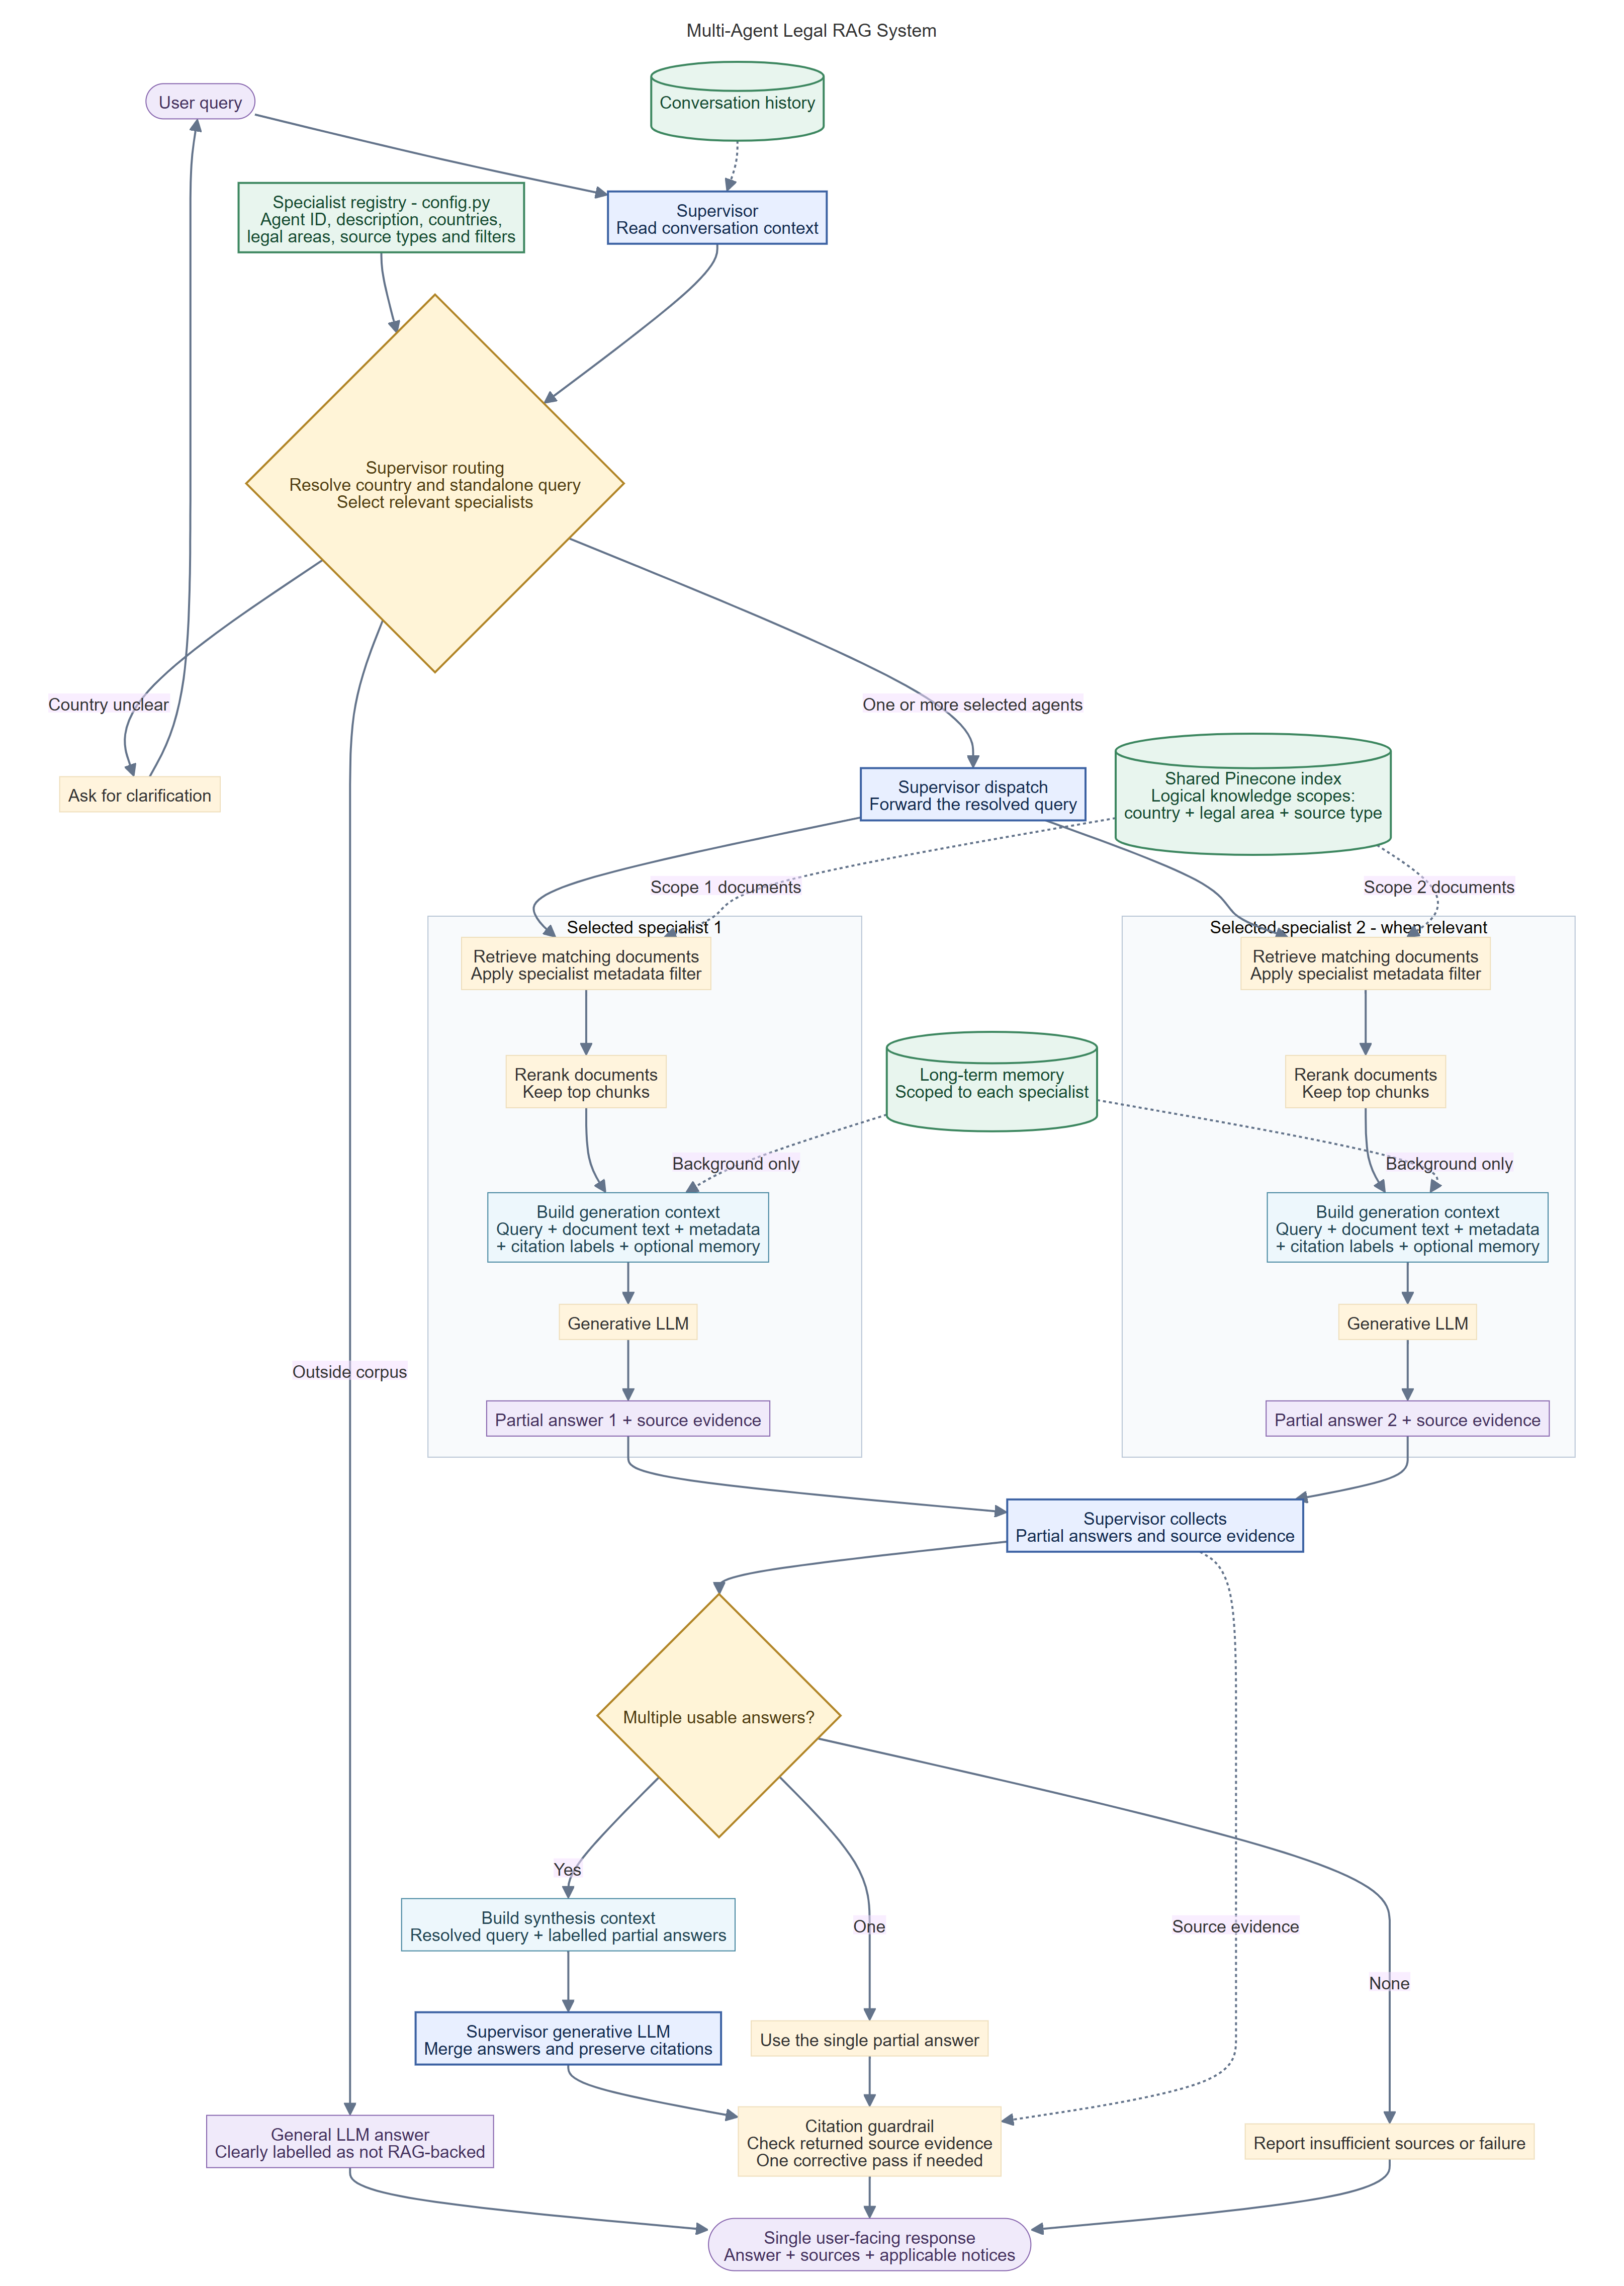
\includegraphics[
        width=\textwidth,
        height=0.85\textheight,
        keepaspectratio
    ]{immagini/multi-agent-system.png}
    \caption{MultiAgentRag workflow.}
    \label{fig:multi-agent-architecture}
\end{figure}
\clearpage

\subsection{Construction of Specialist Contexts}

Each specialist embeds the resolved query and performs a filtered
similarity search, retrieving up to twenty candidate chunks. A
cross-encoder reranks them, and the top five are considered for context
construction. Usable chunks are assembled with source metadata and
unambiguous citation labels.

The generation context contains the resolved question and retrieved
evidence. It may also include summaries of similar past interactions,
recalled from long-term memory using the specialist's identifier.
These summaries provide conversational background, not documentary
evidence.

The language model generates a partial answer citing the supplied
sources. Each specialist returns a structured result containing its
identifier, answer, labelled evidence, retrieved-document metadata,
and relevance score.

\subsection{Collection and Synthesis of Partial Answers}

The supervisor collects usable specialist results. A single partial
answer is used directly; multiple answers are passed to a synthesis
model. If none are usable, the system reports insufficient sources
or an execution failure.

The synthesis context contains the resolved query and labelled partial
answers, without reassembling the retrieved chunks. The model merges
the contributions while preserving citations, combining findings
within each jurisdiction and organizing cross-country answers
comparatively. Source evidence remains separately available for
citation verification and reporting.

\subsection{Citation Verification and Final Response}

An output guardrail checks whether cited evidence supports the
associated statements in the retrieval-backed answer. It checks up to
ten claim--citation pairs per pass and allows one corrective rewrite
followed by verification. Notices report unresolved citation issues
or incomplete checks. This assesses citation support without
guaranteeing the accuracy of every assertion.

The supervisor appends source information and any separately labelled
external-country answer, then saves the response to conversation
history and short-term memory. The retrieval-backed portion may also
be summarized into long-term memory through a background task.
External-country answers bypass corpus-based citation verification
and are excluded from long-term storage.





\section{Multi-Agent Architecture and Main Modules}
\label{sec:overall_architecture}

MultiAgentRag separates configuration management, query routing,
answer generation, and response verification into dedicated modules.
A central supervisor coordinates specialized agents covering divorce
and inheritance law in Italy, Estonia, and Slovenia. As described
previously, document ingestion is shared with the single-agent
implementation. The multi-agent system accesses the resulting
Pinecone index through specialist-specific metadata filters.

\subsection{Configuration Management}

The \path{config.py} module defines the specialist registry.
Each entry specifies an agent's identifier, natural-language
description, jurisdiction, legal areas, source types, and retrieval
filter. Descriptions guide agent selection, while filters restrict
the evidence available to each specialist.

The registry contains eleven specialists: four each for Italy and
Slovenia, and three for Estonia. Legislation and case law are handled
separately for each legal area, except for Estonian inheritance law,
which uses a combined specialist.

The \path{llm_client.py} module centralizes provider configuration
and model assignments for answer generation, citation verification,
and memory summarization. Credentials and provider selection are
loaded from environment settings, while retrieval models and
concurrency parameters are defined in \path{agents.py}.

\subsection{Query Rewriting and Routing}

The \path{ask()} method of \path{SupervisorAgent} coordinates
the online workflow. Through the \path{routing.py} module, it uses
recent conversation context to rewrite context-dependent requests
as standalone questions, resolve the jurisdiction, and select
relevant specialists. These operations are performed within a
single language-model call.

The routing result is validated against the user's messages.
Missing or ambiguous jurisdictions trigger clarification before
retrieval, preventing the system from automatically extending
an unspecified request to all supported countries.

Conversational requests can receive direct responses without
retrieval. Questions concerning countries outside the corpus
receive general language-model answers, explicitly labelled
as not supported by retrieved sources. Mixed requests combine
a corpus-based answer for supported countries with a separately
labelled answer for external countries.

\subsection{Answer Generation}

The supervisor sends the same resolved query to the selected
specialists, with up to four executing concurrently. Each
specialist's \path{answer()} method embeds the query and retrieves
up to twenty candidate chunks from Pinecone using its configured
metadata filter. A cross-encoder reranks these candidates, and
the top five are considered for context construction.

The generation context combines the resolved question with usable
source passages, metadata, and citation labels. It may also include
summaries of similar past interactions recalled from long-term
memory for the selected specialist. These summaries provide
conversational background and are not treated as documentary
evidence. The language model produces a partial answer, returned
alongside its source evidence, document metadata, and relevance
score.

A single usable partial answer proceeds directly to verification.
When several are available, the supervisor constructs a synthesis
context from the resolved query and partial answers. The synthesis
model combines their contributions while preserving citations,
using a comparative structure when multiple jurisdictions are
involved. Retrieved passages remain separately available for
verification rather than being included again in the synthesis
context. If no usable partial answers are returned, the system
reports insufficient sources or an execution failure.

\subsection{Verification and Interaction Management}

The \path{guardrails/output_guard.py} module checks whether cited
sources support their associated claims. It evaluates up to fourty 
claim--citation pairs per pass and permits one corrective rewrite,
followed by another verification pass. Unresolved citation issues
and incomplete checks are reported through notices. This process
assesses citation support rather than guaranteeing the accuracy
of every statement.

The supervisor appends source information and any external-country
answer, then saves the completed response to conversation history
and short-term memory. A background process may summarize the
retrieval-backed portion for long-term semantic memory.
External-country answers bypass corpus-based citation verification
and are excluded from long-term storage.

The \path{ui.py} module provides the Gradio interface for submitting
questions, inspecting source information, and managing conversations.

























\chapter{LangChain RAG Implementation}

The LangChain-based single-agent and multi-agent systems share the
same document ingestion pipeline and legal corpus. The dataset is
unchanged from the previous implementations and covers divorce and
inheritance law in Italy, Estonia, and Slovenia.

LangChain was introduced to explore how its modular interfaces
affect code organization, component integration, and reuse while
preserving the overall system architectures. A further objective
was to investigate how a different embedding model influences
retrieval quality and, consequently, the generated answers.
Access to a rented GPU server on Paperspace enabled experiments
with more computationally demanding embedding models. These
experiments examine both implementation choices and embedding
performance; changes in answer quality should therefore not be
attributed to LangChain alone.

\subsubsection{Document Preparation and Embedding Generation}

The pipeline validates the input JSON documents and standardizes
their metadata, including country, legal area, document type, and
source. Each document receives a citation label for source
attribution.

Using the tokenizer associated with NVIDIA's
\texttt{Nemotron-3-Embed-1B-BF16}, documents are divided into chunks
of up to 1,500 tokens with a 150-token overlap; shorter documents
remain intact. This overlap limits context loss, although chunk
boundaries may still divide sentences or legal provisions.

Chunks are enriched with metadata before a shared LangChain
adapter generates normalized, 2,048-dimensional embeddings on a
CUDA GPU. Passages and queries use the prefixes \texttt{passage:}
and \texttt{query:}, respectively, with consistent model and
preprocessing settings across ingestion and retrieval.

\subsubsection{Vector Storage and Retrieval Integration}

Embeddings are stored in a shared Pinecone index using cosine
similarity, alongside the original chunk text, metadata, citation
label, and chunk position. Records and index dimensions are
validated before batch uploads, which include retries for transient
failures. Deterministic identifiers prevent duplicate records when
unchanged documents are re-ingested, while a local manifest
records the ingestion configuration and document and vector counts.

The single-agent system derives retrieval filters from the query;
the multi-agent system applies filters according to each
specialist's scope. Using the same corpus and vector
representations allows the comparison to focus on differences
in routing, retrieval, and answer generation.


\section{LangChain single Agent Workflow}
\section{Single-Agent Workflow}

Figure~\ref{fig:langchain-single-agent} illustrates the single-agent
workflow: the system interprets the question, selects retrieval
filters, retrieves and reranks relevant passages, and generates
an answer whose citations are checked before storage and delivery.
The LangChain and non-LangChain implementations share essentially
the same architecture. Their differences are primarily at the
implementation level: LangChain provides standardized interfaces
and composable processing stages, while the embedding model also differs.
\clearpage
\begin{figure}[p]
    \centering
    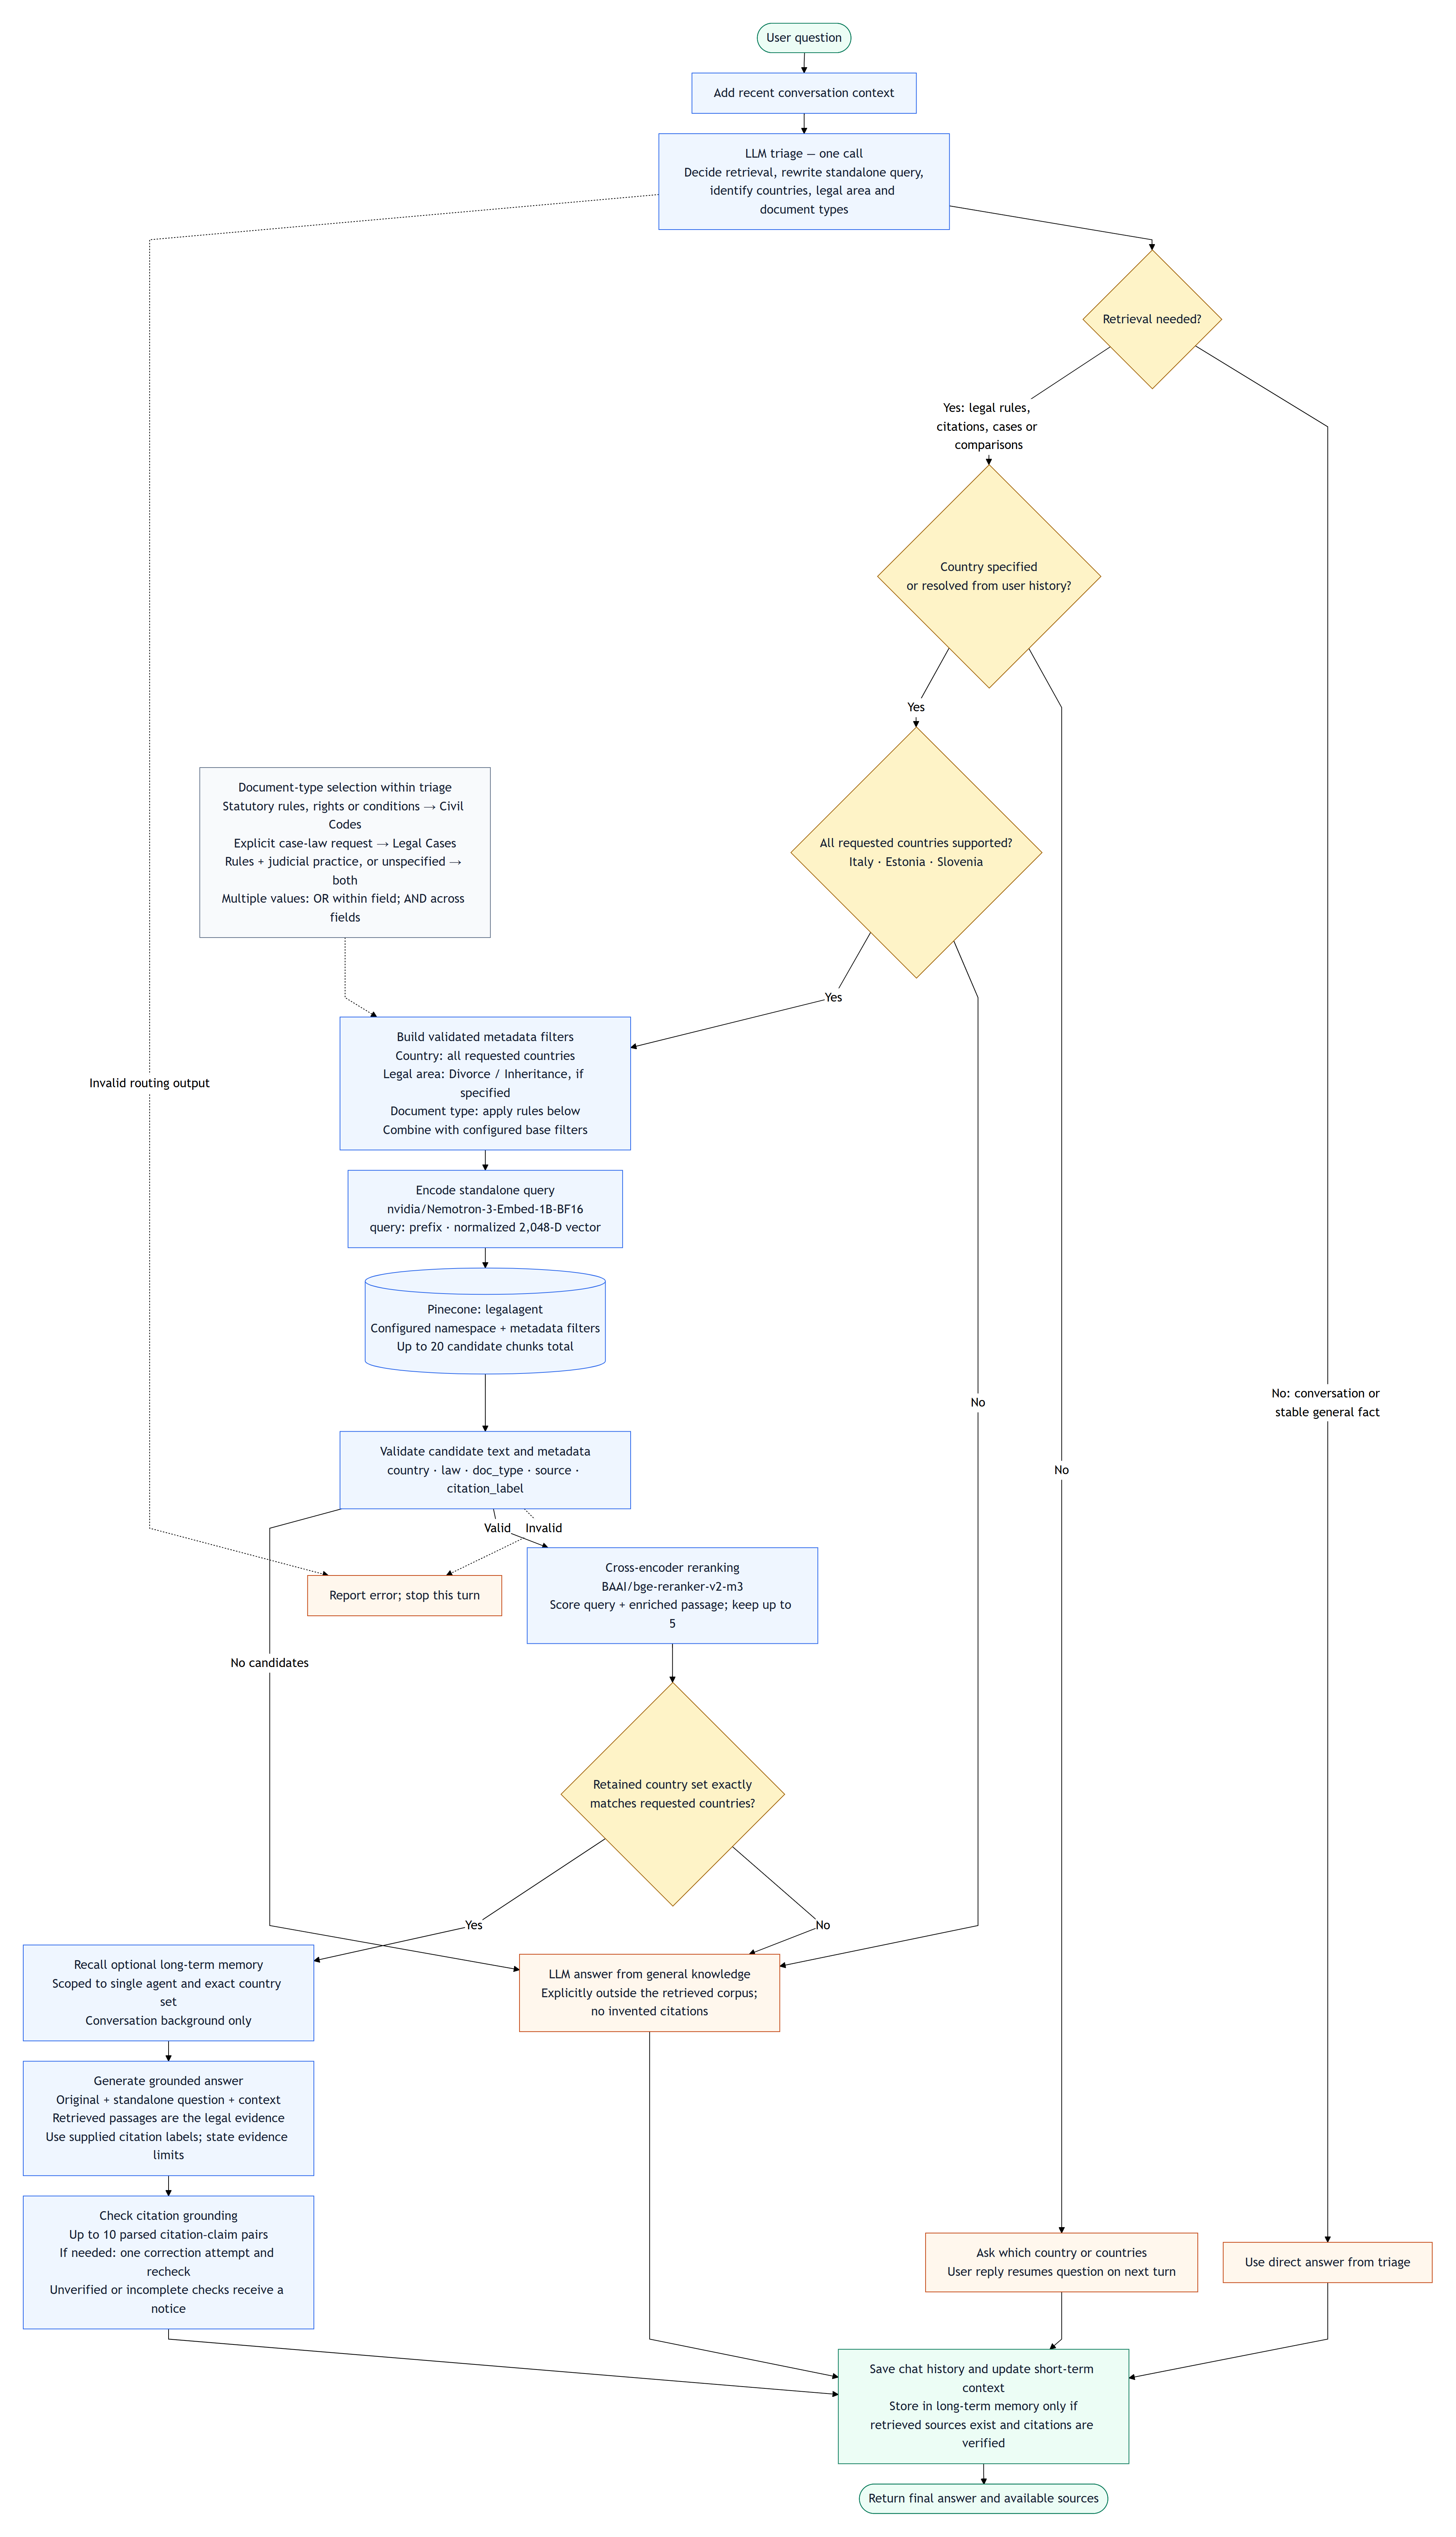
\includegraphics[
        width=\textwidth,
        height=0.85\textheight,
        keepaspectratio
    ]{immagini/langchain_single_agent.png}
    \caption{LangChain single-agent workflow.}
    \label{fig:langchain-single-agent}
\end{figure}
\clearpage

\section{Overall Architecture}

\subsubsection{Workflow Orchestration}

The main change introduced by LangChain concerns the organization
and orchestration of the code. In the original implementation,
\texttt{agent.py} coordinates the processing stages through
explicit procedural calls. In the LangChain version,
\texttt{agent.ipynb} composes these stages using
\texttt{RunnableLambda} and \texttt{RunnableBranch}. The former
wraps operations such as routing, retrieval, generation, and
persistence; the latter selects between alternative paths,
including direct responses, retrieval-grounded answers, and
general-knowledge fallback.

\subsubsection{Model and Retrieval Interfaces}

The component interfaces are also standardized.
\texttt{llm\_client.ipynb} initializes native LangChain chat models,
allowing the agent to invoke different providers through a common
interface. Similarly, \texttt{retrieval.ipynb} implements a
LangChain retriever that combines query embedding, filtered
Pinecone search, and reranking. Retrieved passages are returned
as \texttt{Document} objects, keeping their text and metadata
together as they pass through the workflow.

\subsubsection{Citation Verification, Memory, and User Interface}

The remaining notebooks preserve the original responsibilities.
\texttt{output\_guard.ipynb} exposes citation verification as a
runnable, while \texttt{short\_term.ipynb},
\texttt{long\_term.ipynb}, and \texttt{chat\_history.ipynb}
manage recent context, persistent semantic memory, and conversation
records, respectively. These modules are loaded by
\texttt{agent.ipynb} and connected to the user interface in
\texttt{ui.ipynb}.

\subsubsection{Architectural Continuity and Embedding Changes}

LangChain changes how the existing components are implemented
and composed, rather than introducing a fundamentally different
architecture. The replacement of BGE-M3 with Nemotron in the
embedding stage is a separate experimental choice, intended
to investigate its effect on retrieval and answer quality.


\section{LangChain Multi-Agent Workflow}

The LangChain-based system follows the same overall workflow as the
previous multi-agent implementation: a supervisor selects relevant
legal specialists, forwards the query, and combines their cited
partial answers into a single response. The main difference lies
in the implementation, which uses LangChain interfaces to integrate
the components.
\clearpage
\begin{figure}[p]
    \centering
    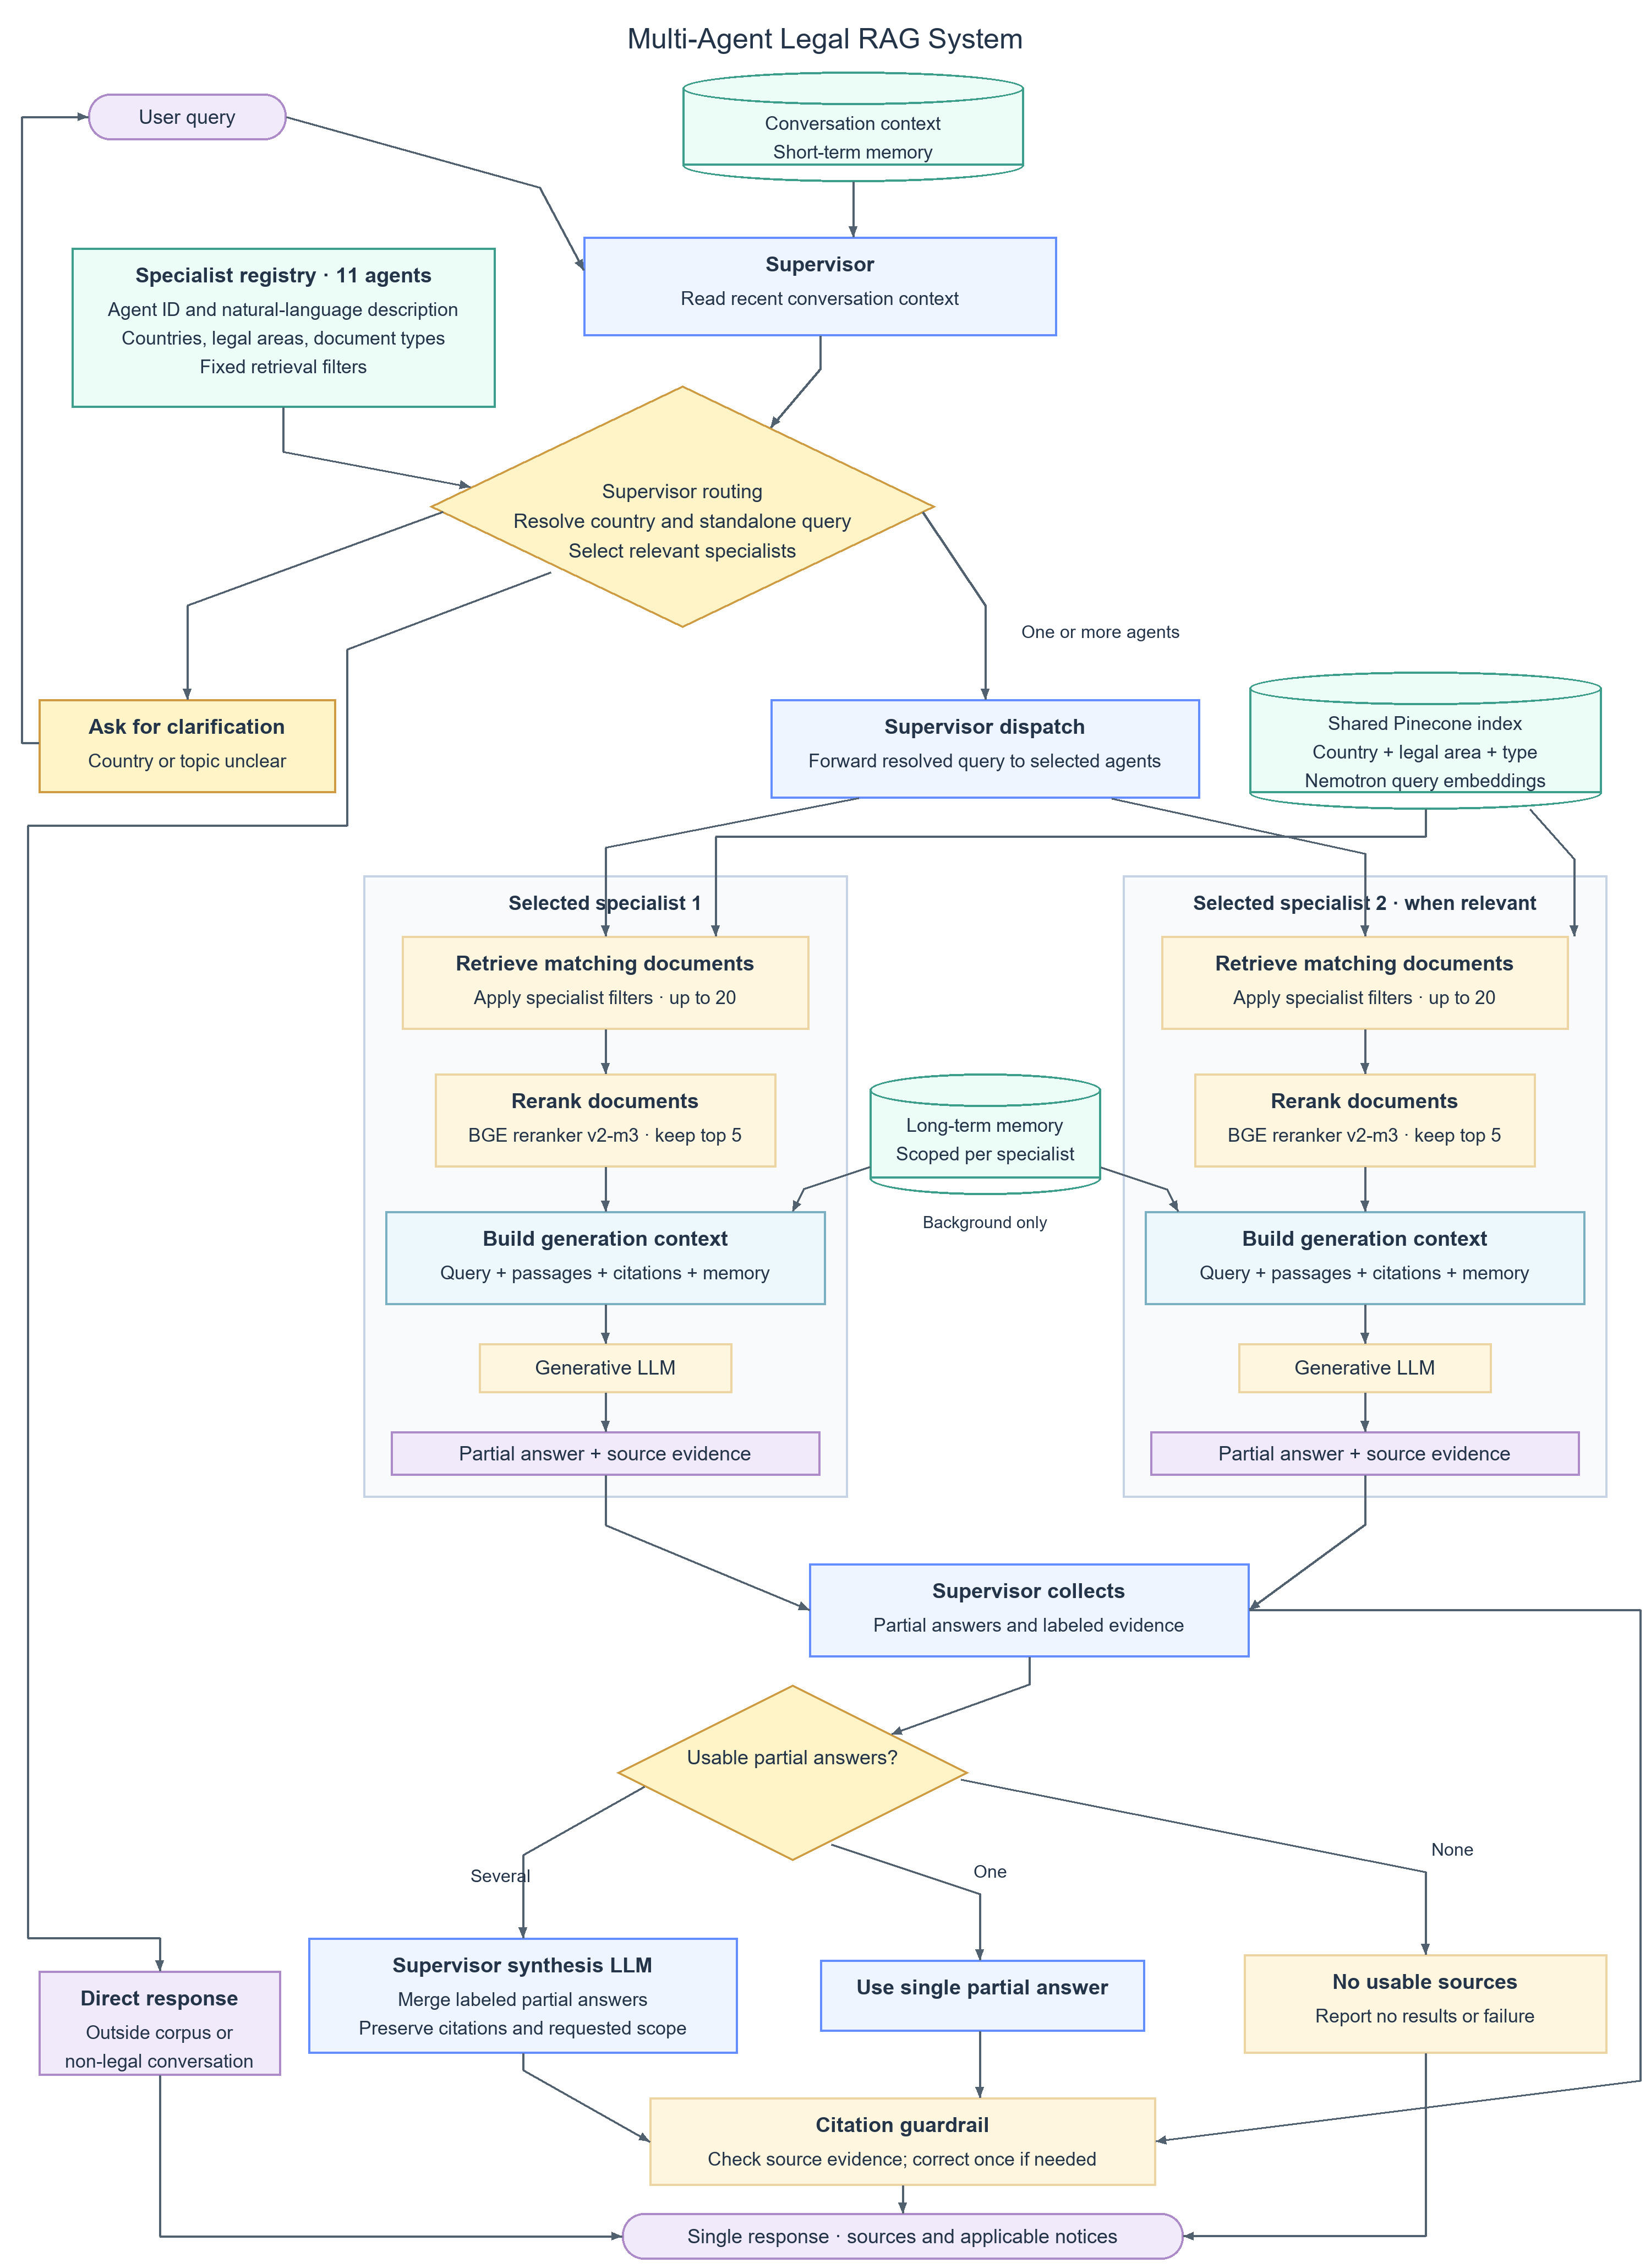
\includegraphics[
        width=\textwidth,
        height=0.85\textheight,
        keepaspectratio
    ]{immagini/langchain_multi_agent_style2.png}
    \caption{LangChain multi-agent workflow.}
    \label{fig:langchain-multi-agent-architecture}
\end{figure}
\clearpage



\section{Overall Architecture}

The system employs a modular multi-agent architecture that separates shared infrastructure, specialist knowledge, and workflow coordination.

\subsection{Infrastructure and Specialist Registry}

At the foundational level, a centralized configuration module manages API credentials, language-model selection, token limits, and connections to the embedding model, reranker, and vector database. This shared infrastructure ensures consistency across agents while allowing individual components to be updated independently. A specialist registry describes the available agents by defining their jurisdictions, legal domains, supported document types, role descriptions, and metadata filters. The registry therefore provides the supervisor with the information required to select the most appropriate specialists for each request.

\subsection{Orchestration and Pipeline Routing}

The workflow is orchestrated by the \texttt{SupervisorAgent.ask()} method, which acts as the main entry point to the system. It receives the user's message, loads the relevant conversation history, and coordinates the answer-generation process. Its first stage, \texttt{\_triage\_and\_route()}, analyses the current request together with the preceding dialogue and selects one of three pipelines.

The direct-answer pipeline handles conversational or general requests that do not require documentary evidence, thereby avoiding unnecessary retrieval. The clarification pipeline is activated when the request is ambiguous or lacks information required for reliable routing. In this case, the supervisor asks a focused follow-up question instead of selecting a specialist based on incomplete information. The user's reply is subsequently combined with the stored history to construct a precise, self-contained query.

\subsection{Specialist Retrieval and Answer Generation}

For domain-specific questions requiring supporting evidence, the supervisor activates the specialist retrieval pipeline. After identifying the relevant legal areas or jurisdictions, it invokes \texttt{\_dispatch\_agents()} to forward the standalone query to one or more specialists. Each specialist then executes its own \texttt{answer()} pipeline: it applies domain-specific metadata filters, searches the vector store for semantically relevant passages, reranks the retrieved candidates, and selects the strongest evidence that fits within the model's context window. Based on this evidence, the specialist produces a partial answer in which substantive claims are linked to source citations.

\subsection{Synthesis, Validation, and Memory}

When several specialists are involved, their outputs are processed by \texttt{\_aggregate()}, which removes unnecessary repetition and combines complementary findings into a coherent final response while preserving citations. If only one usable specialist answer is returned, it passes through directly, avoiding an additional generation step that could introduce information loss. If the available documents do not provide sufficient evidence, the system returns a qualified response rather than presenting an unsupported conclusion.

Before delivery, \texttt{check\_grounding()} verifies that the main claims are supported by the retrieved passages and that the citations are consistent with their sources. Finally, the request and response are stored in conversational memory, allowing later interactions to resolve references, preserve context, and improve routing decisions.







































\chapter{Evaluation Metrics and Conclusion}

\section{Evaluation Methodology}
\label{sec:evaluation_methodology}

The four RAG implementations were evaluated using a common procedure
based on the Ragas framework. Five complementary metrics were selected
to assess the quality of retrieved information and generated answers:
\textbf{Context precision}, \textbf{context recall}, \textbf{faithfulness}, \textbf{answer relevancy},
and \textbf{answer correctness}. All systems were evaluated using the same
DeepSeek judge model, configuration, and BGE-M3 embedding model to
maintain consistent scoring conditions.

The evaluation dataset consisted of questions paired with reference
answers. For each question, the corresponding RAG system generated a
response and retrieved supporting document passages. The question,
reference answer, generated response, and retrieved passages were
stored in an evaluation record. Reference answers were used only
during scoring and were not provided to the systems when generating
their responses.

Each question was processed in a new session, with long-term memory
disabled, to prevent information from previous evaluation cases from
influencing subsequent answers. The experiment therefore assessed
independent question answering rather than multi-turn conversational
performance.

Data collection and scoring were performed as separate stages.
This allowed previously collected responses and passages to be
rescored without rerunning the RAG pipelines. The evaluator was
configured with temperature zero to reduce variability, although
LLM-based judgments are not guaranteed to be fully deterministic.

\section{Evaluation Metrics}
\label{sec:evaluation_metrics}

\paragraph{Context precision.}
Context precision measures whether retrieved passages judged relevant
to the reference answer appear early in the retrieval order.
The implemented metric, \texttt{LLMContextPrecisionWithReference},
uses the evaluator to assign a relevance judgment to each passage.
The score is calculated as
\[
\mathrm{ContextPrecision}
=
\frac{\sum_{k=1}^{K} P(k)\,v_k}
     {\sum_{k=1}^{K} v_k},
\qquad
P(k)=\frac{\sum_{i=1}^{k}v_i}{k},
\]
where $K$ is the number of retrieved passages and $v_k$ is one
when passage $k$ is judged relevant and zero otherwise.
The expression assumes at least one relevant passage.
A high score indicates that relevant passages are concentrated
near the beginning of the saved retrieval order.

For the multi-agent systems, passages are combined in agent registry
order, followed by each agent's internal retrieval order.
Consequently, this metric evaluates the saved combined order rather
than a globally reranked list of passages.

\paragraph{Context recall.}
Context recall measures the extent to which the retrieved passages
support the information contained in the reference answer.
The reference is decomposed into claims, and the evaluator determines
whether each claim can be supported by the retrieved context:
\[
\mathrm{ContextRecall}
=
\frac{\text{Number of reference claims supported by the context}}
     {\text{Total number of reference claims}}.
\]
A high score indicates that retrieval provides evidence covering
most of the expected answer. This is a measure of reference-claim
coverage, rather than document recall over the entire corpus.

\paragraph{Faithfulness.}
Faithfulness measures whether the claims made in the generated
response are supported by the retrieved passages:
\[
\mathrm{Faithfulness}
=
\frac{\text{Number of response claims supported by the context}}
     {\text{Total number of response claims}}.
\]
Unlike context recall, faithfulness examines claims in the generated
response rather than claims in the reference answer. It does not
directly depend on the reference.

A high score indicates that the answer is grounded in the retrieved
evidence. However, it does not establish that the evidence itself
is accurate or that the response contains all information needed
to answer the question.

\paragraph{Answer relevancy.}
Answer relevancy assesses how closely the generated response
addresses the original question. Ragas generates a set of questions
from the response and compares their embeddings with the embedding
of the original question using cosine similarity. Responses judged
noncommittal are penalized.

This metric does not use the reference answer directly. A high
score indicates that the response addresses the requested topic,
but does not necessarily establish factual accuracy or completeness.

\paragraph{Answer correctness.}
Answer correctness compares the generated response with the
reference answer through a combination of factual agreement and
semantic similarity:
\[
\mathrm{AnswerCorrectness}
=
0.75\,F + 0.25\,S,
\]
where $F$ represents the factual comparison component and $S$
represents embedding-based semantic similarity.

The factual component compares claims in the response and reference,
accounting for matching claims, additional unmatched claims, and
missing reference claims. The semantic component measures similarity
in meaning. The score therefore reflects agreement with the selected
reference rather than an independent verification of every statement
against external sources.

\section{Influence of Reference-Answer Quality}
\label{sec:reference_quality}

Reference-answer design is an essential part of the evaluation.
Context precision, context recall, and answer correctness depend
directly on the reference answer. Faithfulness and answer relevancy
do not use it directly and provide complementary perspectives on
response quality.

A reference answer defines the expected content and level of detail.
A concise reference establishes a narrow target, whereas a more
detailed reference may introduce additional facts, conditions, or
exceptions. Changing these expectations can alter the scores even
when the generated response and retrieved passages remain unchanged.


\section{Aggregation and Interpretation}
\label{sec:evaluation_interpretation}

Scores were calculated separately for each question and then
aggregated using the arithmetic mean of valid numerical results:
\[
\overline{m}
=
\frac{1}{|V_m|}
\sum_{i \in V_m} m_i,
\]
where $V_m$ is the set of cases with a valid score for metric $m$.

Generation failures were excluded from scoring. When no passages
were retrieved, context precision, context recall, and faithfulness
were left unscored, while answer relevancy and answer correctness
could still be evaluated. Scoring failures were also excluded from
the corresponding metric mean. 

The five metrics must be interpreted jointly. High faithfulness with low context recall indicates an answer based on incomplete evidence, while high context recall with low answer correctness suggests relevant evidence was retrieved but poorly utilized. Furthermore, high answer relevancy alone doesn't ensure correctness. Even combining high faithfulness with high answer relevancy only proves the LLM perfectly processed the provided context it does not guarantee a factually complete or correct final answer if the retrieved information itself is flawed.

\section{Ragas Results}
In this section, we present the evaluation results for the four RAG implementations, highlighting their performance across the five selected metrics. 

Each implementation was evaluated using the same set of test questions and ground-truth references. Specifically, we compare the performance differences between single-agent and multi-agent architectures, as well as the impact of using different embedding models contrasting a lightweight model with a higher-parameter alternative.

\subsection{Performance Comparison}

% Nel preambolo:
% \usepackage{graphicx}
% \usepackage{multirow}

\begin{table}[htbp]
    \centering
    \caption{Evaluation results of the four RAG implementations.}
    \label{tab:rag_evaluation}

    \resizebox{\textwidth}{!}{%
        \begin{tabular}{llccccc}
            \hline
            \textbf{Embedding Model} &
            \textbf{Architecture} &
            \textbf{Faithfulness} &
            \textbf{Context Recall} &
            \textbf{Answer Rel.} &
            \textbf{Context Prec.} &
            \textbf{Answer Corr.} \\
            \hline

            \multirow{2}{*}{BGE (568M)}
            & Multi-Agent & 0.958 & 0.442 & 0.604 & 0.595 & 0.433\\
            & Single-Agent  & 0.856 & 0.225 & 0.622 & 0.276 & 0.551 \\
            \hline

            \multirow{2}{*}{Nemotron (1B)}
            & Single-Agent & 0.971 & 0.335 & 0.716 & 0.630 & 0.501 \\
            & Multi-Agent  & 0.989 & 0.371 & 0.757 & 0.568 & 0.518 \\
            \hline
        \end{tabular}%
    }
\end{table}
\begin{sloppypar}
To ensure a consistent comparison, all four configurations were
evaluated using \texttt{deepseek-chat} as the Ragas evaluator and
\texttt{BAAI/bge-m3} as the embedding model. Gemini was initially
tested as an alternative evaluator. However, the free-tier request
limit was exceeded because Ragas requires multiple API calls per
sample. After paid API access was enabled, the project's monthly
spending cap was reached before a single evaluation run could be
completed. DeepSeek was therefore retained for all experiments,
as its available quota supported the evaluation workload.
\end{sloppypar}

\subsubsection{General Considerations}

Multi-agent architectures can outperform single-agent systems on complex research tasks by distributing the workload among specialized agents. Each agent can focus on a particular argument, topic, source type, or country, allowing it to develop deeper and more contextually relevant knowledge. This specialization can also improve document retrieval and source organization: instead of producing a single, heterogeneous collection of references, the system can retrieve and organize sources separately for each topic or country. A coordinating agent can then compare the findings, reconcile inconsistencies, and synthesize the results into a coherent final response.

However, multi-agent systems also introduce additional computational costs and coordination overhead. Their use is therefore most beneficial when a task can be divided into clearly defined subtasks that lend themselves to parallel processing or require specialized analysis.

Although the benefits may not be immediately evident from the quantitative results alone, the integration of \textbf{BGE-M3} and \textbf{Nemotron} improved the system's overall performance, particularly in terms of reasoning, instruction following, document retrieval, and the quality of intermediate outputs. To illustrate these qualitative improvements, the following section compares two responses to the same predefined question. The first response was generated by our multi-agent pipeline, which uses \textbf{BGE-M3} for document retrieval and \textbf{Nemotron} for language generation and reasoning. The second was produced by \textbf{Gemini} using its free API tier.

Evaluating both systems on the same question enables a direct comparison of their depth of analysis, relevance, source selection and organization, and overall response quality. The complete responses and a detailed comparison supporting the observations discussed above are available at the following link: \href{run:./multiagent-model-answer-comparison.pdf}{response comparison}.
\end{document}